\documentclass{article}

\usepackage[left=4cm, right=4cm]{geometry}
\usepackage{palatino}%Fuente
\usepackage{eulervm}%Fuente
\usepackage{graphicx}%Imágenes
\usepackage{float}%Imágenes
\usepackage{subcaption}%Imágenes
\usepackage{enumitem}%Listas
\usepackage{parskip}%Espacio entre párrafos
\usepackage{multicol}
\usepackage{amsthm,thmtools,xcolor}
\usepackage{amssymb}%Mate
\usepackage{amsmath}%Mate
\usepackage{tikz}%Mate (diagramas)
\usepackage{dutchcal}
\usepackage{tikz-cd}
\usepackage{xcolor}
\definecolor{blue-violet}{rgb}{0.54, 0.17, 0.89}
\usetikzlibrary{%
	matrix,%
	calc,%
	arrows,%
	shapes,
	decorations.markings,backgrounds,calc,intersections
}
\usepackage[bookmarks,bookmarksopen,bookmarksdepth=3]{hyperref}
\usepackage{cleveref}
\hypersetup{%colores
	colorlinks=true,
	urlcolor=blue,
	linkcolor=magenta,
	citecolor=blue,
	filecolor=blue,
	urlbordercolor=white,
	linkbordercolor=white,
	citebordercolor=white,
	filebordercolor=white
}

\makeatletter %Hide section number
\def\@seccntformat#1{%
	\expandafter\ifx\csname c@#1\endcsname\c@section\else
	\csname the#1\endcsname\quad
	\fi}
\makeatother
\usepackage{sectsty}
\sectionfont{\fontsize{13}{20}\selectfont}

\usepackage[style=authortitle,backend=bibtex]{biblatex}
\addbibresource{complex-geometry.bib}

\definecolor{blue-violet}{rgb}{0.54, 0.17, 0.89}
\definecolor{azure}{rgb}{0.0, 0.5, 1.0}
\definecolor{green(ncs)}{rgb}{0.0, 0.62, 0.42}
\definecolor{forestgreen}{rgb}{0.13, 0.55, 0.13}
\definecolor{limegreen}{rgb}{0.2, 0.8, 0.2}
\definecolor{palatinateblue}{rgb}{0.15, 0.23, 0.89}
\definecolor{trueblue}{rgb}{0.0, 0.45, 0.81}
\definecolor{goldenyellow}{rgb}{1.0, 0.87, 0.0}
\definecolor{fashionfuchsia}{rgb}{0.96, 0.0, 0.63}
\definecolor{brightcerulean}{rgb}{0.11, 0.67, 0.84}
\definecolor{jonquil}{rgb}{0.98, 0.85, 0.37}
\definecolor{lavendermagenta}{rgb}{0.93, 0.51, 0.93}
\definecolor{peru}{rgb}{0.8, 0.52, 0.25}
\definecolor{persimmon}{rgb}{0.93, 0.35, 0.0}
\definecolor{persianred}{rgb}{0.8, 0.2, 0.2}
\definecolor{persianblue}{rgb}{0.11, 0.22, 0.73}
\definecolor{persiangreen}{rgb}{0.0, 0.65, 0.58}
\definecolor{persianyellow}{rgb}{0.9, 0.89, 0.0}

\theoremstyle{definition}

\declaretheoremstyle[headfont=\color{trueblue}\normalfont\bfseries,]{colored1}
\declaretheoremstyle[headfont=\color{forestgreen}\normalfont\bfseries,]{colored2}
\declaretheoremstyle[headfont=\color{peru}\normalfont\bfseries,]{colored3}
\declaretheoremstyle[headfont=\color{persiangreen}\normalfont\bfseries,]{colored4}
\declaretheoremstyle[headfont=\color{brightcerulean}\normalfont\bfseries,]{colored5}
\declaretheoremstyle[headfont=\color{lavendermagenta}\normalfont\bfseries,]{colored6}
\declaretheoremstyle[headfont=\color{blue-violet}\normalfont\bfseries,]{colored7}
\declaretheoremstyle[headfont=\color{green(ncs)}\normalfont\bfseries,]{colored8}
\declaretheoremstyle[headfont=\color{peru}\normalfont\bfseries,]{colored9}
\declaretheoremstyle[headfont=\color{persiangreen}\normalfont\bfseries,]{colored10}

\declaretheorem[style=colored1,numberwithin=section,name=Theorem]{thm}
\declaretheorem[style=colored2,numberwithin=section,numberlike=thm,name=Proposition]{prop}
\declaretheorem[style=colored3,numberwithin=section,numberlike=thm,name=Lemma]{lemma}
\declaretheorem[style=colored4,numberwithin=section,numberlike=thm,name=Corollary]{coro}
\declaretheorem[style=colored5,numbered=no,name=Example]{example}
\declaretheorem[style=colored5,numbered=no,name=Examples]{examples}
\declaretheorem[style=colored6,numbered=no,name=Exercise]{exercise}
\declaretheorem[style=colored7,numberwithin=section,name=Remark]{remark}
\declaretheorem[style=colored7,numberwithin=section,name=Observation]{obs}
\declaretheorem[style=colored9,numbered=no,name=Claim]{claim}
\declaretheorem[style=colored8,numbered=no,name=Definition]{defn}
\declaretheorem[style=colored10,numbered=no,name=Question]{question}

\numberwithin{equation}{section}

\newcommand{\A}{\mathbb{A}}
\newcommand{\R}{\mathbb{R}}
\newcommand{\Z}{\mathbb{Z}}
\newcommand{\N}{\mathbb{N}}
\newcommand{\C}{\mathbb{C}}
\newcommand{\Q}{\mathbb{Q}}
\newcommand{\D}{\mathbb{D}}
\renewcommand{\P}{\mathbb{P}}

\newcommand{\Ac}{\mathcal{A}}
\newcommand{\Bc}{\mathcal{B}}
\newcommand{\Cc}{\mathcal{C}}
\newcommand{\Dc}{\mathcal{D}}
\newcommand{\Ec}{\mathcal{E}}
\newcommand{\Fc}{\mathcal{F}}
\newcommand{\Gc}{\mathcal{G}}
\newcommand{\Hc}{\mathcal{H}}
\newcommand{\Ic}{\mathcal{I}}
\newcommand{\Jc}{\mathcal{J}}
\newcommand{\Kc}{\mathcal{K}}
\newcommand{\Lc}{\mathcal{L}}
\newcommand{\Mc}{\mathcal{M}}
\newcommand{\Nc}{\mathcal{N}}
\newcommand{\Oc}{\mathcal{O}}
\newcommand{\Pc}{\mathcal{P}}
\newcommand{\Qc}{\mathcal{Q}}
\newcommand{\Rc}{\mathcal{R}}
\newcommand{\Sc}{\mathcal{S}}
\newcommand{\Tc}{\mathcal{T}}
\newcommand{\Uc}{\mathcal{U}}
\newcommand{\Vc}{\mathcal{V}}
\newcommand{\Wc}{\mathcal{W}}
\newcommand{\Xc}{\mathcal{X}}
\newcommand{\Yc}{\mathcal{Y}}
\newcommand{\Zc}{\mathcal{Z}}

\newcommand{\mf}{\mathfrak{m}}
\newcommand{\Cinf}{C^\infty}

\DeclareMathOperator{\img}{img}
\DeclareMathOperator{\Arg}{Arg}
\DeclareMathOperator{\id}{id}
\DeclareMathOperator{\Alt}{Alt}
\DeclareMathOperator{\Spec}{Spec}
\DeclareMathOperator{\sgn}{sgn}
\DeclareMathOperator{\supp}{supp}
\DeclareMathOperator{\Int}{Int}
\DeclareMathOperator{\Ob}{Ob}
\DeclareMathOperator{\Mor}{Mor}
\DeclareMathOperator{\Top}{Top}
\DeclareMathOperator{\CGWH}{CGWH}
\DeclareMathOperator{\Hom}{Hom}
\DeclareMathOperator{\Map}{Map}
\DeclareMathOperator{\Tot}{Tot}
\DeclareMathOperator{\Vect}{Vect}
\DeclareMathOperator{\VectBund}{VectBund}
\DeclareMathOperator{\Open}{Open}
\DeclareMathOperator{\Ring}{Ring}
\DeclareMathOperator{\Set}{Set}
\DeclareMathOperator{\Sets}{Sets}
\DeclareMathOperator{\Ab}{Ab}
\DeclareMathOperator{\op}{op}
\DeclareMathOperator{\Groups}{Groups}
\DeclareMathOperator{\eq}{eq}
\DeclareMathOperator{\Fun}{Fun}
\DeclareMathOperator{\Coh}{Coh}
\DeclareMathOperator{\coker}{coker}
\DeclareMathOperator{\an}{an}
\DeclareMathOperator{\alg}{alg}
\DeclareMathOperator{\Pic}{Pic}
\DeclareMathOperator{\GL}{GL}
\DeclareMathOperator{\SL}{SL}
\DeclareMathOperator{\SO}{SO}
\DeclareMathOperator{\U}{U}
\DeclareMathOperator{\SU}{SU}
\DeclareMathOperator{\Sp}{Sp}
\DeclareMathOperator{\M}{M}
\DeclareMathOperator{\Aut}{Aut}
\DeclareMathOperator{\PGL}{PGL}
\DeclareMathOperator{\PSL}{PSL}


\begin{document}
{\Huge complex geometry}
\tableofcontents
\section{abstract nonsense}

\begin{defn}\leavevmode
	\begin{itemize}
		\item A \textbf{\textit{pullback}} of the morphisms $f$ and $g$ consists of an object $P$ and two morphisms $p_1:P\to X$ and $p_2:P\to Y$ satisfying the following universal property:
		\[\begin{tikzcd}
			Q\arrow[rrd,bend left,"q_2"]\arrow[ddr,"q_1",swap,bend right]\arrow[dr,dashed,"\phi"]\\
			&P\arrow[r,"p_2"] \arrow[rd, phantom, "\lrcorner", very near start]\arrow[d,"p_1",swap]&Y\arrow[d,"g"]\\
			&X\arrow[r,"f",swap]&Z
		\end{tikzcd}\]
		\item A \textbf{\textit{pushout}} of the morphisms $f$ and $g$ consists of an object $P$ and two morphisms $i_1:P\to X$ and $i_2:P\to Y$ satisfying the following universal property:
		\[\begin{tikzcd}
			Z\arrow[r,"g"]\arrow[d,swap,"f"]&Y\arrow[d,"i_2"]\arrow[ddr,bend left,"j_2"]\\
			X\arrow[r,"i_1",swap]\arrow[drr,bend right,swap,"j_1"]&P\arrow[ul, phantom, "\ulcorner", very near start]\arrow[dr,dashed,"\phi"]\\
			&&Q
		\end{tikzcd}\]
		\item A \textbf{\textit{product}} of $X$ and $Y$ is an object $X\sqcup Y$ and a pair of morphisms $p_1:X\sqcap Y\to X$, $p_2:X\sqcap Y\to Y$ satisfying the following universal property:
		\[\begin{tikzcd}
			Q\arrow[rrd,bend left,"q_2"]\arrow[ddr,"q_1",swap,bend right]\arrow[dr,dashed,"\phi"]\\
			&X\sqcap Y\arrow[r,"p_2"]\arrow[d,"p_1",swap]&Y\\
			&X
		\end{tikzcd}\]
		\item A \textbf{\textit{coporoduct}} of $X$ and $Y$ is an object $X\sqcup Y$ and a pair of morphisms $i_1:X\to X\sqcup Y$, $i_2:Y\to X\sqcup Y$ satisfying the following universal property:
		\[\begin{tikzcd}
			&Y\arrow[d,"i_2"]\arrow[ddr,bend left,"j_2"]\\
			X\arrow[r,"i_1",swap]\arrow[drr,bend right,swap,"j_1"]&X\sqcup Y\arrow[dr,dashed,"\phi"]\\
			&&Q
		\end{tikzcd}\]
		\item A morphism $i$ has the \textbf{\textit{left lifting property with respect to a morphism $p$}} and $p$ has the \textbf{\textit{right lifting property with respect to $i$}} if for each morphisms $f$ and $g$, if the outer square in the following diagram commutes, there exists $\phi$ (I think not necessarily unique) completing the diagram:
		\[\begin{tikzcd}[row sep=large]
			A\arrow[r,"f"]\arrow[d,"i",swap]&X\arrow[d,"p"]\\
			B\arrow[r,"g",swap]\arrow[ur,dashed,"\phi"]&Y
		\end{tikzcd}\]
		\item The \textbf{\textit{kernel}} of a morphism is that part of its domain which is sent to zero. Formally, in a category with an initial object 0 and pullbacks, the \textbf{\textit{kernel $\ker f$}} of a morphism $f:A\to B$ is the pullback $\ker(f)\to A$ along $f$ of the unique morphism $0\to B$
		
		More explicitly, this characterizes the object $\ker(f)$ as \textit{the} object (unique up to isomorphism) that satisfies the following universal property:
		\begin{quote}
			for every object $C$ and every morphism $h:C\to A$ such that $f\circ h=0$ is the zero morphism, there is a unique morphism $\phi:C\to\ker(f)$ such that $h=p\circ\phi$.
		\end{quote}
		\[\begin{tikzcd}
			C\arrow[dr,dashed,"\phi"]\arrow[ddr,bend right,swap,"h"]\\
			&\ker(f)\arrow[d]\arrow[r]&0\arrow[d]\\
			&A\arrow[r,"f",swap]&B\arrow[ul, phantom, "\ulcorner", very near start]
		\end{tikzcd}\]
		\item In a category with a terminal object 1, the \textbf{\textit{cokernel}} of a morphism $f:A\to B$ is the pushout (arrows $h$ and $\phi$ apply if terminal object is zero)
		\[\coker(f):=1\sqcup_AB\qquad\qquad\begin{tikzcd}
			A\arrow[r,"f"]\arrow[d]\arrow[dr, phantom, "\lrcorner", very near start]&B\arrow[d]\arrow[rdd,bend left,"h"]\\
			1\arrow[r]&\coker(f)\arrow[dr,dashed,"\phi"]\\
			&&C
		\end{tikzcd}\]
		In the case when the terminal object is in fact zero object, one can, more explicitly, characterize the object $\coker(f)$ with the following universal property:
		\begin{quote}
			for every object $C$ and every morphism $h:B\to C$ such that $h\circ f=0$ is the zero morphism, there is a unique morphism $\phi:\coker(f)\to C$ such that $h=\phi\circ i$.
		\end{quote}
		
		\item A morphism $f:X\to Y$ is a \textbf{\textit{monomorphism}} if for every object $Z$ and every pair of morphisms $g_1,g_2:Z\to X$ then
		\[f\circ g_1=f\circ g_2\implies g_1=g_2.\]
		\[\begin{tikzcd}
			Z\arrow[r,shift={(0,.06)},"g_1"]\arrow[r,swap,shift={(0,-.06)},"g_2"]\arrow[rr,bend left,"f\circ g_1"]\arrow[rr,bend right,swap,"f\circ g_2"]&X\arrow[r,"f"]&Y
		\end{tikzcd}\]
		Equivalently, $f$ is a monomorphism if for every $Z$ the hom-functor $\Hom(Z,-)$ takes it to an injective function
		\[\begin{tikzcd}
			\Hom(Z,X)\arrow[r,hook,"f_*"]&\Hom(Z,Y).
		\end{tikzcd}\]
		Being a monomorphism in a category $\Cc$ means equivalently that it is an epimorphism in the opposite category $\Cc^{\op}$.
		
		\item A morphism $f:X\to Y$ is a \textbf{\textit{epimorphism}} if for every object $Z$ and every pair of morphisms $g_1,g_2:Y\to Z$ then
		\[g_1\circ f=g_2\circ f\implies g_1=g_2.\]
		\[\begin{tikzcd}
			X\arrow[r,"f"]\arrow[rr,bend right,swap,"g_2\circ f"]\arrow[rr,bend left,"g_1\circ f"]&Y\arrow[r,shift={(0,.06)},"g_1"]\arrow[r,swap,shift={(0,-.06)},"g_2"]&Z
		\end{tikzcd}\]
		Equivalently, $f$ is a epimorphism if for every $Z$ the hom-functor $\Hom(-,Z)$ takes it to an injective function
		\[\begin{tikzcd}
			\Hom(Y,Z)\arrow[r,hook,"f^*"]&\Hom(X,Z).
		\end{tikzcd}\]
		Being a monomorphism in a category $\Cc$ means equivalently that it is an monomorphism in the opposite category $\Cc^{\op}$.
	\end{itemize}
\end{defn}
\section{sheaf cohomology}
Let's read \cite{huybrechts}, appendix B.

In the following, $M$ will be a topological space. In most of the examples it is a differential or complex manifold.
\begin{defn}
	A \textbf{\textit{pre-sheaf $\Fc$}} of abelian groups (or vector spaces, rings, etc.) on $M$ consists of an abelian group (resp. vecot space, ring, etc.) $\Gamma(U,\Fc)=\Fc(U)$ for every open subset $U\subset M$ and a group homomorphism (resp. linear map, ring homomorphism, etc.) $r_{U,V}:\Fc(V)\to \Fc(U)$ for any two nested open subsets $U\subset V$ satisfying the following two conditions:
	\begin{enumerate}
		\item[$(i)$] $r_{U,U}=\id_{\Fc(U)}$.
		\item[$(ii)$] For open subsets $U\subset V\subset W$ one has $r_{U,V}\circ r_{V,W}=r_{U,V}$.
	\end{enumerate}
	Sometimes, one additionally requires $\Fc(\varnothing)=0$. In order to lighten the notation a bit, one may also write $s|_U$ instead of $r_{U,V}(s)$.
\end{defn}
\begin{example}
	The basic example is $\Fc=\Cc_M^0$, the pre-sheaf of continuous functions on $M$. More precisely, $\Cc_M^0(U)$ is the ring of all continuous maps $f:U\to\R$.
\end{example}
For $\Fc=\Cc_M^0$ one easily verifies the following additional conditions which do not hold for arbitrary pre-sheaves. We let $U=\bigcup U_i$ be the union of open subsets $U_i\subset M$. Then 
\begin{enumerate}
	\item[$(iii)$] If $f,g\in\Cc^0_M\left(\bigcup U_i\right)$ with $r_{U_i,U}(f)=r_{U_i,U}(g)$ for all $i$, then $f=g$.
	\item[$(iv)$] If functions $f_i\in\Cc_M^0(U_i)$ are given for all $i$ such that $r_{U_i\cap U_j,U_i}(f_i)=r_{U_i\cap U_j,U_j}(f_j)$ for any $j$, then there exists a continuous function $f\in\Cc^0_M(U)$ with $r_{U_i,U}(f)=f_i$ for all $i$.
\end{enumerate}
This leads to the definition of a sheaf.

\begin{defn}
	A pre-sheaf $\Fc$ is called a \textbf{\textit{sheaf}} if $(iii)$ and $(iv)$ are satisfied.
\end{defn}
\begin{examples}\leavevmode
	\begin{itemize}
		\item The constant pre-sheaf $\R$, for which $\Fc(U)=\R$ for all open subsets $\varnothing\neq U\subset M$ is not a sheaf as soon as $M$ contains a disconnected open subset. So, one works rather with the \textbf{\textit{constant sheaf(!) $\underline{\R}$}}, which, on an open set $U\subset M$ yields the set of all continuous functions $f:U\to\R$, where $\R$ is endowed with the discrete topology.
	
		Of course, one defines in the same manner constant sheaves associated to other vector spaces, groups, rings, etc.
		\item Another important example is the sheaf $\Ec$ of sections of a (topological) vector bundle $\pi:E\to M$. By definition, $\Ec(U)$ is the set of all (continuous) maps $s:U\to E$ with $\pi\circ s=\id_U$.
		
		In fact $\Ec$ is sheaf of $\Cc_M^0$-modules, that is, each $\Ec(U)$ is a $\Cc_M^0(U)$-module and the restriction maps are comparible with the module structures on the different open subsets.
		
		Since the vector bundle $E$ can be recovered from its sheaf of sections $\Ec$, one often uses the same notation $E$ for both.
	\end{itemize}
\end{examples}

\begin{defn}
	Let $\Fc$ and $\Gc$ be two (pre-)sheaves. A \textbf{\textit{(pre-)sheaf homomorphism}} $\varphi:\Fc\to\Gc$ is given by group homomorphisms (linear maps, ring homomorphisms, etc.) $\varphi_U:\Fc(U)\to\Gc(U)$ for any open subset $U\subset M$ satisfying $r_{U,V}^{\Gc}\circ \varphi_V=\varphi_U\circ r_{U,V}^{\Fc}$ for any $U\subset V$.
\end{defn}
Once a homomorphism $\varphi:\Fc\to \Gc$ of (pre-)sheaves of abelian groups is given, one constructs the associated pre-sheaves $\ker(\varphi)$, $\img(\varphi)$ and $\coker(\varphi)$ which are defined in the obvious way, that is, $\coker(\varphi)(U)=\coker(\varphi_U:\Fc(U)\to\Gc(U))$.

There is an important subtlety here. If $\varphi$ is a sheaf homomorphism then $\ker(\varphi)$ is a sheaf itself, but $\img(\varphi)$ and $\coker(\varphi)$, in general, are just pre-sheaves. In order to define the cokernel and the image of a sheaf homomorphism as honest sheaves, one needs to introduce the notion of a stalk.
\begin{defn}
	Let $\Fc$ be a (pre-)sheaf on $M$ and $x\in M$. Then the \textbf{\textit{stalk}} of $\Fc$ at $x$ is
	\[\Fc_x:=\{(U,s):x\in U\subset M,s\in\Fc(U)\}/\sim\]
	Here, for two open subsets $U_i$, $i=1,2$ and sections $s_i\in\Fc(U_i)$, $i=1,2$, one sets $(U_1,s_1)\sim(U_2,s_2)$ if there exists an open subset $x\in U\subset U_1\cap U_2$ such that $r_{U,U_1}(s_1)=r_{U,U_2}(s_2)$.
	
	Equivelently, one could introduce the stalk $\Fc_x$ as the direct limit $\Fc_x=\lim_{x\in U}\Fc(U)$.
\end{defn}
\begin{remark}
	One immediatly finds that any section $s\in\Fc(U)$ induces an element $s_x\in\Fc_x$ for any point $x\in U$. Furthermore, any (pre-)sheaf homomorphism $\varphi:\Fc\to\Gc$ induces homomorphisms $\Fc_x\to\Gc_x$ for any $x\in M$.
\end{remark}
\begin{defn}
	The \textbf{\textit{sheaf $\Fc^+$ associated to a pre-sheaf $\Fc$}} is the sheaf for which $\Fc^+(U)$ of an open subset $U\subset M$ is the set of all maps $s:U\to\bigcup_{x\in U}\Fc_x$ with $s(x)\in\Fc_x$ and such that for all $x\in U$ there exists an open subset $x\in V\subset U$ and a section $t\in\Fc(V)$ with $s(y)=t(y)$ for all $y\in V$. {\color{magenta}what?}
\end{defn}
\begin{remark}
	With this definition, $\Fc^+$ is a sheaf and the natural inclusion $\Fc\subset\Fc^+$ is an isomorphism if the pre-sheaf $\Fc$ was already a sheaf. For many constructions one needs to pass from a naturally defined pre-sheaf to its \textbf{\textit{sheafification}}. For example, the tensor product $\Fc\otimes_{\Rc}\Gc$ of two $\Rc$-modules $\Fc$ and $\Gc$ is defined as the sheafification of $U\mapsto\Fc(U)\otimes_{\Rc(U)}\Gc(U)$.
\end{remark}

\begin{defn}
	Let $\varphi:\Fc\to\Gc$ be a homomorphism of sheaves. Then the \textbf{\textit{image sheaf $\img(\varphi)$}} is the sheaf associated with the image pre-sheaf $U\mapsto\img(\varphi_U)$. Analogously, one defines the \textbf{\textit{cokernel sheaf $\coker(\varphi)$}}.
\end{defn}
\begin{defn}
	The sheaf homomorphism $\varphi$ is \textbf{\textit{injective}} if and only if $\ker(\varphi)$ is trivial. Similarly, one says that $\varphi$ is \textbf{\textit{surjective}} if its cokernel sheaf $\coker(\varphi)$ is trivial.
\end{defn}
	The essential difference between the two properties is that $\varphi$ is injective if and only if $\varphi_U$ is injective for any open set $U$. On the other hand, $\varphi$ might be surjective without $\varphi_U$ being surjective for all/any open subset. However, both properties can be detected by ther stalks. More precisely,
\begin{quote}
	$\varphi$ is injective or surjective if and only if $\varphi_x:\Fc_x\to\Gc_x$ is injective respectively surjective for any point $x\in M$.
\end{quote}
\begin{defn}
	A sequence $\Fc^\bullet$ of sheaf homomorphisms
	\[\begin{tikzcd}
		\cdots\arrow[r]&\Fc^i\arrow[r,"\varphi^i"]&\Fc^{i+1}\arrow[r,"\varphi^{i+1}"]&\Fc^{i+2}\arrow[r,"\varphi^{i+2}"]&\cdots
	\end{tikzcd}\]
	is a \textbf{\textit{complex}} if $\varphi^{i+1}\circ\varphi^i=0$ for all $i$. It is in an \textbf{\textit{exact complex}} if $\ker\varphi^{i+1}=\img\varphi^i$ for all $i$.
	
	An exact complex of the form \begin{tikzcd}
		0\arrow[r]&\Fc^0\arrow[r]&\Fc^1\arrow[r]&\Fc^2\arrow[r]&0
	\end{tikzcd} is called \textbf{\textit{short exact sequence}}.
\end{defn}
\begin{coro}
	A complex of the form
	\[\begin{tikzcd}
		0\arrow[r]&\Fc^0\arrow[r]&\Fc^1\arrow[r]&\Fc^2\arrow[r]&0
	\end{tikzcd}\]
	is exact if and only if the induced complex of stalks
	\[ \begin{tikzcd}
		0\arrow[r]&\Fc_x^0\arrow[r]&\Fc_x^1\arrow[r]&\Fc_x^2\arrow[r]&0
	\end{tikzcd}\]
	is exact for any $x\in M$.
\end{coro}
\begin{remark}
	Since surjectivity does not mean surjectivity for any open subset, a short exact sequence as above does not necessarily define short exact sequences
	\[ \begin{tikzcd}
		0\arrow[r]&\Fc^0(U)\arrow[r]&\Fc^1(U)\arrow[r]&\Fc^2(U)\arrow[r]&0
	\end{tikzcd}\]
	for any subset $U\subset M$ and in particular not for $M$. \textbf{This is where cohomology comes in.} It turns out that the failure of surjectivity of $\Fc^1(M)\to\Fc^2(M)$ is measured by the cohomology of $\Fc^0$.
\end{remark}

In order to introduce sheaf cohomology, one has to make a choice. There is the theoretically superior but rather abstract approach via derived categories or the more ad hoc one using acyclic resolutions. We outline the second one.

One first has to single out special sheaves with no cohomology in order to define cohomology for all other ones by resolving them.

\begin{defn}
	A \textbf{\textit{resolution}} of a sheaf $\Fc$ is a complex  \begin{tikzcd}
		0\arrow[r]&\Fc^0\arrow[r]&\Fc^1\arrow[r]&\Fc^2\arrow[r]&0
	\end{tikzcd} together with a homomorphism $\Fc\to\Fc^0$ such that
	\[\begin{tikzcd}
		0\arrow[r]&\Fc\arrow[r]&\Fc^0\arrow[r]&\Fc^1\arrow[r]&\Fc^2\arrow[r]&\cdots
	\end{tikzcd}\]
	is an exact complex of sheaves.
\end{defn}
One possible choice for sheaves without cohomology is provided by flasque sheaves.
\begin{defn}
	A sheaf $\Fc$ is called \textbf{\textit{flasque}} if for any open subset $U\subset M$ the restriction map $r_{U,M}:\Fc(M)\to\Fc(U)$ is surjective.
\end{defn}
Why flasque sheaves are the right ones is explained by the following
\begin{lemma}\label{lem:flasque}
	If
	\[\begin{tikzcd}
		0\arrow[r]&\Fc^0\arrow[r]&\Fc^1\arrow[r]&\Fc^2\arrow[r]&0
	\end{tikzcd}\]
	is a short exact sequence and $\Fc^0$ is flasque, then the induced sequence
	\[\begin{tikzcd}
		0\arrow[r]&\Fc^0(U)\arrow[r]&\Fc^1(U)\arrow[r]&\Fc^2(U)\arrow[r]&0
	\end{tikzcd}\]
	is exact for any open subset $U\subset M$.
\end{lemma}
Next, one has to ensure that any sheaf can be resolved by flasque sheaves. This will allow to define the cohomology of any sheaf.
\begin{prop}\label{prop:flasque-resolutions}
	Any sheaf $\Fc$ on $M$ admits a resolution
	\[\begin{tikzcd}
		0\arrow[r]&\Fc\arrow[r]&\Fc^0\arrow[r]&\Fc^1\arrow[r]&\Fc^2\arrow[r]&\cdots
	\end{tikzcd}\]
	such that all sheaves $\Fc^i$, $i=0,1,\ldots$ are flasque.
\end{prop}
\begin{defn}
	The \textbf{\textit{$i$-th cohomology group $H^i(M,\Fc)$}} of a sheaf $\Fc$ is the $i$-th cohomology of the complex
	\[\begin{tikzcd}
		\Fc^0(M)\arrow[r,"\varphi^0"]&\Fc^1(M)\arrow[r,"\varphi^1"]&\Fc^2(M)\arrow[r,"\varphi^2"]&\cdots
	\end{tikzcd}\]
	{\color{cyan}induced by a flasque resolution} $\Fc\to\Fc^\bullet$. Explicitly,
	\[H^i(M,\Fc)=\dfrac{\ker(\varphi^i_M:\Fc^i(M)\to\Fc^{i+1}(M))}{\img(\varphi^{i-1}_M:\Fc^{i-1}(M)\to\Fc^i(M))}\]
\end{defn}
Clearly, with this definition any flasque sheaf $\Fc$ has vanishing cohomology $H^i(M,\Fc)=0$ for $i>0$. (This is because of \cref{lem:flasque}: though it is stated as a \textit{short} exact sequence, it certainly implies exactness at every arrow in a long exact sequence of flasque sheaves.)

Moreover, for any sheaf $\Fc$ one has $\ker\varphi_M^0=H^0(M,\Fc)=\Gamma(M,\Fc)=\Fc(M)$. Indeed, in virtue of \cref{prop:flasque-resolutions}, \[\img(\Fc\to\Fc^0)=\ker(\Fc^0\to\Fc^1)\]
as sheaves, that is, as the sheafifications of the pre-sheaves
\[U\mapsto\img (\varphi_U:\Fc(U)\to\Fc^0(U))\quad \text{and}\quad U\mapsto\ker(\varphi^0_U:\Fc^0(U)\to\Fc^1(U))\]
calling the first arrow $\varphi$ for now. Taking $U=M$, we simply have that
\[\img\varphi_M=\ker\varphi^0_M\]
and $\varphi_M:\Fc(M)\to\Fc^0(M)$ injectively so that $\img\varphi_M\cong\Fc(M)$.

That this definition of cohomology is really independent of the chosen fiasque resolution is due to
\begin{prop}
	If $\Fc\to\Fc^\bullet$ and $\Fc\to\Gc^\bullet$ are two flasque resolutions of a sheaf $\Fc$ then both define naturally isomorphic cohomology groups.
\end{prop}

The most striking feature of cohomology is that it explains fully the non­ exactness of short exact sequences on the level of global sections.
\begin{prop}
	Let
	\[\begin{tikzcd}
		0\arrow[r]&\Fc^0\arrow[r]&\Fc^1\arrow[r]&\Fc^2\arrow[r]&0
	\end{tikzcd}\]
	be a short exact sequence of sheaves on $M$. Then there exists a \textbf{\textit{long exact cohomology sequence}}
	\[\begin{tikzcd}
		0\arrow[r]&H^0(M,\Fc^0)\arrow[r]&H^0(M,\Fc^1)\arrow[r]&H^0(M,\Fc^2)\arrow[dll]\\
		&H^1(M,\Fc^0)\arrow[r]&H^1(M,\Fc^1)\arrow[r]&H^1(M,\Fc^2)\arrow[dll]\\
		&H^2(M,\Fc^0)\arrow[r]&H^2(M,\Fc^1)\arrow[r]&H^2(M,\Fc^2)\arrow[r]&\cdots
	\end{tikzcd}\]
\end{prop}
\begin{defn}
	Suppose $\Fc$ is a sheaf {\color{cyan}of vector spaces} on $M$. Then $h^i(M,\Fc)$ denotes the dimension of $H^i(M,\Fc)$, which inherits a natural vector space structure. If all $h^i(M,\Fc)$ are finite and only finitely many are non-trivial we say $\Fc$ has \textbf{\textit{finite cohomology}} and we define the \textbf{\textit{Euler-Poincaré characteristic of $\Fc$}} as
	\[\chi(M,\Fc):=\sum(-1)^ih^i(M,\Fc).\]
\end{defn}
\begin{remark}
	In \cite{hatcher-at}, we have the following result for a finite CW complex $Y$:
	\[\sum_{i=0}^\infty(-1)^i(\#i-\text{cells})=\sum_{i=0}^\infty(-1)^i\operatorname{ran}H_i(Y;\Z),\]
	where left-hand side is defined as the Euler-Poincaré characteristic $\chi(Y)$.
\end{remark}
\begin{coro}
	Let
	\[\begin{tikzcd}
		0\arrow[r]&\Fc^0\arrow[r]&\Fc^1\arrow[r]&\Fc^2\arrow[r]&0
	\end{tikzcd}\]
	be a short exact sequence of sheaves of vector spaces with finite cohomology. Then
	\[\chi(M,\Fc^1)=\chi(M,\Fc^0)+\chi(M,\Fc^2).\]
\end{coro}
It might happen that flasque resolutions are difficult to find. But in order to compute the cohomology of a sheaf, any resolution by \textbf{\textit{acyclic sheaves}}, i.e. sheaves with trivial higher cohomology groups, can be used. What kind of acyclic sheaves are convenient depends on the situation. For topological, differentiable, and complex manifolds, the following one is very useful. For the Zariski topology one has to use different ones.
\begin{defn}
	A sheaf $\Fc$ is called \textbf{\textit{soft}} is the restriction $\Gamma(M,\Fc)\to\Gamma(K,\Fc)$ is surjective for any closed subset $K\subset M$.
	
	The space of sections $\Gamma(K,\Fc)$ of $\Fc$ over the closed set $K$i\textit{is defined} as the direct limit of the spaces of sections over all open neighbouthoods of $K$.
\end{defn}
\begin{prop}
	Soft sheaves are acyclic. Any sheaf of modules over a soft sheaf of commutative rings is soft and hence acyclic.
\end{prop}
\begin{remark}
	This is frequently applied to the sheaf of continuous (or differentiable) functions on a manifold \textit{which is easily shown to be soft}. Notice that the sheaf of holomorphic functions on a complex manifold \textit{is not soft}.
\end{remark}

\textbf{\textit{\v Chech cohomology}} is another cohomology theory. It has the advantage to be defined without any sheaf resolution. Since it often coincides with the cohomology defined above, we will sketch the main steps of its construction.

Let us first fix an open covering $M=\bigcup_iU_i$ with $I$ an order set and consider the intersections $U_{i_0\ldots i_p}:=U_{i_0}\cap\ldots\cap U_{i_p}$. Then we set
\[C^p(\{U_i\},\Fc)=\prod_{i_0<\ldots<i_p}\Gamma(U_{i_0\ldots i_p},\Fc)\]
{\color{cyan}(It doesn't seem to be a very meaningful definition… I would rather like it if they were formal sums of something like in \cref{remark:chain-complexes})} There is a natural differential
\begin{align*}
	d:C^p(\{U_i\},\Fc)&\to C^{p+1}(\{U_i\},\Fc)\\
	\alpha=\prod\alpha_{i_0\ldots i_p}&\mapsto d\alpha
\end{align*}
with
\[(d\alpha)_{i_0\ldots i_{p+1}}=\sum_{k=0}^{p+1}(-1)^k\alpha_{i_0\ldots\widehat{i_k}\ldots i_{p+1}}|_{U_{i_0\ldots i_p+1}}\]
\begin{remark}\label{remark:chain-complexes}
	Recall from \cite{hatcher-at} that a \textbf{\textit{singular $n$-simplex}} in a space $X$ is by definition just a map $\sigma:\Delta^n\to X$. The word 'singular' is used here to express the idea that $\sigma$ need not be a nice embedding but can have 'singularities' where its image does not look at all like a simplex. All that is required is that $\sigma$ be continuous. Let $C_n(X)$ be the free abelian group with basis the set of singular $n$-simplices in $X$. Elements of $C_n(X)$, called \textbf{\textit{$n$-chains}}, are finite formal sums $\sum_in_i\sigma_i$ for $n_i\in\Z$ and $sigma_i:\Delta^n\to X$. A boundary map $\partial_n:C_n(X)\to C_{n-1}(X)$ is defined by specifying its values on the basis elements:
	\[\partial_n(\sigma)=\sum_i(-1)^i\sigma|[v_0,\ldots,\widehat{v_i},\ldots,v_n],\]
	which intuitively means that the boundary of the $n$-simplex consists of various ordered $(n-1)$-dimensional simplices, where the symbol $\hat{}$ over $v_i$ indicates that this vertex is deleted from the sequence $v_0,\ldots,v_n$.
	
	Then, given a space $X$ and an abelian group $G$, we define the group $C^n(X;G)$ of \textbf{\textit{singular $n$-cochains with coefficients in $G$}} to be the dual group $\Hom(C_n(X),G)$ of the singular chaing group $C_n(X)$. Thus an $n$-cochain $\varphi\in C^n(X;G)$ assigns to each singular $n$-simplex $\sigma:\Delta^n\to X$ a value $\varphi(\sigma)\in G$. Since the singular $n$-simplices form a basis for $C_n(X)$, these values can be chosen arbitrarily, hence $n$-cochains are exactly equivalent to functions from singular $n$-simplices to $G$. A \textbf{\textit{coboundary map}} $\delta:C^n(X;G)\to C^{n+1}(X;G)$ is the dual $\delta^*{\color{cyan}=\Hom(\partial,G)}$, so for a cochain $\varphi\in C^n(X;G)$, its coboundary $\delta\varphi$ is the composition $C_{n+1}(X)\overset{\partial}{\to}C_n(X)\overset{\varphi}{\to}G$.
		\[\begin{tikzcd}
		\textcolor{cyan}{C_{n+1}}\arrow[d,cyan,swap,"\partial"]\arrow[rd,cyan,"\varphi\circ\partial=\partial^*"]\\	\textcolor{cyan}{C_n}\arrow[cyan,swap,r,"\varphi"]&\textcolor{cyan}{G}
	\end{tikzcd}\]
	This means that for a singular $(n+1)$-simplex $\sigma(\Delta^{n+1})\to X$ we have
	\[\varphi\partial (\sigma)=\sum_i(-1)^i\varphi(\sigma|[v_1,\ldots,\widehat{v}_i,\ldots,v_{n+1}])\]
\end{remark}

Back to \cite{huybrechts}, a calculation shows that $d^2=0$, i.e.
\[\begin{tikzcd}
	C^0(\{U_i\},\Fc)\arrow[r,"d"]&C^1(\{U_i\},\Fc)\arrow[r,"d"]&\cdots
\end{tikzcd}\]
is a complex. {\color{magenta}Since $\Fc$ is a sheaf, one finds $\Gamma(M,\Fc)=\ker(d:C^0(\{U_i\},\Fc)\to C^1(\{U_i\},\Fc))$ (I would love to see why…)}.

\begin{defn}
	The \textbf{\textit{$i$-th \v Chech cohomology group}} with respect to the fixe open covering $M=\bigcup_iU_i$ is
	\[\check{H}^i(\{U_i\},\Fc)=\dfrac{\ker(d:C^i(\{U_i\},\Fc)\to C^{i+1}(\{U_i\},\Fc))}{\img(d:C^{i-1}(\{U_i\},\Fc)\to C^i(\{U_i\},\Fc))}\]
	In this way, we have defined cohomology groups without using acyclic sheaves, but which still depend on the open covering $M=\bigcup U_i$. This can be remedied by passing to the limit. More precisely, if $M=\bigcup_i U_i$ is refined by an open covering $M=\bigcup_jV_j$, then there exists a natural map
	\[\check{H}^i(\{U_i\},\Fc)\to\check{H}^i(\{V_j\},\Fc))\]
	and one defines the \v Chech cohomology as a sheaf without specifying an open coveing as
	\[\check{H}^i(M,\Fc):=\lim_\to \check{H}^i(\{U_i\},\Fc).\]
\end{defn}
Now let's quickly do the approach in \cite{donaldson}.
Consider a topological space $X$ and an open cover $X=\bigcup_\alpha U_\alpha$. For simplicity, suppose $X$ is compact and the cover is finite. The \textbf{\textit{nerve}} if the cover is an abstract simplicial complex with one vertes (a 0-simplex) $\sigma_\alpha$ for every open set $U_\alpha$ and a $p$-simplex $\sigma_{\alpha_0,\ldots,\alpha_p}$ for each non-empty intersection $U_{\alpha_0}\cap\ldots\cap U_{\alpha_p}$. Now, given an abelian group $A$, we can form the simplicial cochain complex of this nerve.

For example, a 0-cochain is the assignment of an element $g_\alpha\in A$ to each $U_\alpha$. A 1-cochain assigns an element $g_{\alpha\beta}\in A$. to each non-empty intersection $U_\alpha\cap U_\beta$ and a 2-cochain assigns an element $g_{\alpha\beta\gamma}$ to each non-empty triple intersection $U_\alpha\cap U_\beta\cap U\gamma$. {\color{cyan}(Now this looks much more like \cref{remark:chain-complexes})} We have cochain groups $C^p$ for $p\geq 0$. There is a standar coboundary map $\delta:C^p\to C^{p+1}$. For example, a 1-cochain $\underline{g}=(a_\alpha)$ has $\delta\underline{g}=\underbrace{h}$ where
\[\underline{h}_{\alpha\beta}=g_\alpha-g_\beta\]
and a 2-cochain $\underline{h}$ has $\delta\underline{h}=\underline{k}$, where
\[\underline{k}_{\alpha\beta\gamma}=h_{\alpha\beta}-h_{\alpha\gamma}+h_{\beta\gamma}\]
{\color{cyan}So this is just a way of writing the definition of the boundary map without writing it. So it's not surprising to have a} \textit{Note:} There is an issue about how one handles orientations here; see any book on algebraic topology.

Now we can form the cohomology of this complex $H^*(X;\Uc,A)$, say, where $\Uc$ denotes the open cover. Suppose $X=\bigcup V_i$ is another cover $\Vc$. We say that $\Vc$ is a \textbf{\textit{refinement}} of $\Uc$ if we can choose a map of index sets $\alpha(i)$ such that $V_i$ is contained in $U_{\alpha(i)}$. In this case, we get a natural induced map on cochain complexes and hence a map $H^*(X;\Uc,A)\to H^*(X;\Vc,A)$. The \textbf{\textit{\v Cech cohomology}} $H^*(X,A)$ of $X$ with co-efficients in $A$ is defined by taking the \textbf{\textit{inverse limit}}:

\begin{quote}
	That is, an element of $H^*(X,A)$ is represented by an alement of $H^*(X;\Uc,A)$ for some cover $\Uc$, but two elements represented by $\omega_1\in H^*(X;\Uc_1,A)$, $\omega_2\in H^*(H;\Uc_2,A)$ are equal in $H^*(X;A)$ if there is some common refinement $\Vc$ of $\Uc_1,\Uc_2$ such that $\omega_1,\omega_2$ have the same image in $H^*(X;\Vc,A)$.
\end{quote}
Thus $H^*(X,A)$ is a topological invariant of $X$ and, at least for reasonable spaces such as manifolds, this is in fact isomorphic to the singular cohomology with coefficients in $A$. In practice, one rarely needs to perfom the limiting process explicitly if one works with a sensible cover.

Now, from this standpoint, the generalisation to ‘sheaf cohomology’ is very easy and natural. To keep things simple, for the moment suppose one has a class $S$ of functions on the space $X$ (these could be continuous functions or, if $X$ is a manifold, smooth functions or, if $X$ is a Riemann surface, holomorphic functions). The only property we require is that for each non-emptu open set $U\subset X$ there is a corresponding set $S(U)$ of functions on $U$ of the given class, and if $U\subset U$ we have a restriction map from $S(U)$ to $S(V)$.

We generalise the \v Cech construction by allowing $g_{\alpha_0,\ldots,\alpha_p}$ to ba en element of $S(U_0\cap\ldots\cap U_p)$. The differential $\delta$ is defined by the same formula, but restricting functions on $p+1$ fold intersections to $p$-fold intersections.  Then we get cohomology groups $H^*(X;\Uc,S)$ and, taking limit over coverings, we arrive at an invariant $H^*(X,S)$.

\begin{quote}
	For example, a 0-cochain $\underline{g}$ is given by a function $g_\alpha$ on $U_\alpha$ for each $\alpha$, and the cocycle condition $\delta\underline{g}=0$ asserts that $g_\alpha=g_\beta$ on any non empty intersection $U_\alpha\cap U_\beta$. This just means that the $g_\alpha$ are restrictions of a single function $g$ on $X$. Thus $H^0(X;\Uc,S)=S(X)$.
	
	{\color{cyan}Let us rephrase: a 0-cochain is a formal sum of some holomorphic functions defined on some sets. If this cochain is a cocycle then these functions coincide on the intersections on the sets. Because we are dealing with a sheaf, this means we can make a function on the whole manifold out of the pieces,} {\color{magenta}and then finally I think I am kind of convinced that $H^0(X;\Uc,S)=S(X)$.}
\end{quote}
{\color{cyan}Then we have a discussion on meromorphic functions, definition of a sheaf $\Sc$ on a space $X$, homomorphism of sheaves, injective sheaves, surjective sheaves (which are not what we expect and in fact this is where cohomology came in), and also}
\begin{defn}
	A sheaf $\Sc$ over $M$ is called \textbf{\textit{fine}} if, for each locally finite cover $\{U_i\}$ of $M$ by open sets, there exists for each $i$ an endomorphism $e_i$ of $\Sc$ such that
	\begin{itemize}
		\item $\supp(e_i)\subset U_i$,
		\item $\sum_ie_i=\id$.
	\end{itemize}
	By $\supp$, the \textbf{\textit{support}} of $e_i$ we denote the closure of the set of points $m\in M$ for which $e_i|\Sc_m$ is not zero. We call $\{e_i\}$ a \textbf{\textit{partition of unity}} for $\Sc$ subordinate to the cover $\{U_i\}$ of $M$.
\end{defn}
From our Telegram group (sadly I can't compile the names in Russian…):
\begin{quote}
	\href{https://fr.wikipedia.org/wiki/Faisceau_(mathématiques)#Typologie_des_faisceaux}{Tipologia dos feixes}:
	\begin{itemize}
		\item flabby = flasque
			%=вялый 
			= flácido--- sections extend from open subsets
		\item soft = mou
			%=мягкий 
			= macio--- sections extend from closed subsets
		\item fine = fin
			%=тонкий
	 		= fino--- partition of unity (sheaf of endomorphisms is soft)
	
	And we have:
	
	fine $\implies$ soft $\implies$ flabby $\implies$ acyclic $\implies$ resolutions of this type are useful to compute cohomology
	
	fino $\implies$ macio $\implies$ flácido $\implies$ acíclico $\implies$ útil

	Fine sheaves were introduced by Cartan, flabby and soft by Godement.
	\end{itemize}
\end{quote}

\textbf{Now the basic fact is there is a way to define cohomology groups $H^p(X,\Sc)$ for any sheaf over a space $X$.} Since $X$ is fixed, we will drop it from the notation and just write $H^p(\Sc)$. These can be characterised by the following axioms.
\begin{enumerate}
	\item $H^0(X,\Sc)=\Sc(X)$, the space of \textbf{\textit{global sections}} of $\Sc$.
	\item A sheaf homomorphism $a:\Sc\to\Sc'$ induces homomorphisms from $H^p(X,\Sc)$ to $H^p(X,\Sc')$.
	\item A short exact sequence of sheaves $0\to\Sc\to\Sc'\to\Sc''\to0$ induces a long exact sequence in cohomology
	\[\cdots\to H^p(\Sc')\to H^p(\Sc'')\overset{\delta}{\to}H^{p+1}(\Sc)\to H^{p+1}(\Sc')\to\cdots,\]
	where the boundary maps $\delta$ have an obvious naturality property with respect to homomorphisms of exact sequences.
	\item if $\Sc$ is fine, then $H^p(\Sc)=0$ for $p>0$.
\end{enumerate}

Again from Telegram:
\begin{quote}
	And 'axioms' of Donaldson say merely that $H^p$ are functorial in the sheaf $\Fc$, there is a long exact sequence of cohomology associated with a short exact sequence of sheaves, and fine sheaves are acyclic. First three axioms follow from general formalism of derived functors, fourth gives us a source of sheaves that we can use to construct resolution in order to compute the cohomology (e.g. all sheaves of modules over the sheaf of smooth functions).
\end{quote}

And \cite{donaldson}. One approach is to use the \v Cech construction outlined above to define the groups $H^p(\Sc)$ and then show uniqueness from the axioms. But there are several other approaches, and we refer to more specialised texts for a proper treatment.

\begin{quote}
	{\color{red}\textbf{The point is that however we go about things, we arrive at the same cohomology groups}.}
\end{quote}

Aaaand back to \cite{huybrechts}:
\begin{prop}
	For any open covering $M=\bigcup_iU_i$, there exists an natural homomorphism
	\[\check{H}^i(\{U_i\},\Fc)\to H^i(M,\Fc).\]
\end{prop}
Of course, these homomorphisms are in general not bijective, as the open
covering might be very coarse. However, passing to the limit often results in isomorphism with the true cohomology groups, i.e. when the topological spaces is reasonable (e.g. paracompact), the induced maps $\check{H}^i(M,\Fc)\to H^i(M,\Fc)$ are indeed bijective.
\begin{prop}
	The natural map $\check{H}^1(M,\Fc)\to H^1(M,\Fc)$ is always bijective.
\end{prop}
This opens the way to parametrize line bundles by cohomology classes. Let us sketch this for differentiable real line bundles.

Let $\pi:L\to M$ be a line bundle that can be trivialized over open subsets $U_i$ of an open cover $M=\bigcup U_i$ by maps $\psi_i:L|_{U_i}\cong U_i\times \R$. Then $\{\psi_{ij}:=\psi_i\circ\psi^{-1}_j\in\Cc_M^*(U_i\cap U_j)\}$ {\color{red}can be considered as a cocycle (see \cref{cocycle-condition})} and thus gives rise to an element in $\check{H}^1(\{U_i\},\Cc_M^*)$, where $\Cc^*_M$ is the sheaf of differentiable functions without zeros.

One verifies that this cohomology class does not depend on the choice of the trivializations $\psi_i$. Moreover, any class in $\check{H}^1(\{U_i\},\Cc_M^*)$ can be interpreted as a cocycle of a line bundle trivialized over the open subsets $U_i$.

Thus, by definition every line bundle $L$ gives rise to a cohomology class in the covering independent \v Cech cohomology group $\check{H}^1(M,\Cc^*_M)$ which does not depend neither on the open covering nor on the trivializations. The above proposition then yields

\begin{coro}
	There is a bijection between the set of isomorphism classes of real line bundles on a differentiable manifold $M$ and the group $H^1(M,\Cc^*_M)$.
\end{coro}

{\color{cyan} In sum, since a line bundle can be reconstructed from the gluing maps of the trivializations, and all of those form a cocycle, \textbf{every line bundle is associated to a cocycle!} And it is a bijective correspondence, and that is the Picard group.}

\section{line bundles}
Now let's read some of \cite{hatcher-vb}.

\begin{defn}\leavevmode
	\begin{itemize}
		\item An \textbf{\textit{$n$-dimensional vector bundle}} is a map $p:E\to B$ together with a vector space structure on $p^{-1}(b)$ for each $b\in B$ such that the following local triviality condition is satisfied: there is a cover of $B$ by open sets $U_\alpha$ for each of which there exists a homeomorphism $h_\alpha:p^{-1}(U_\alpha)\to U_\alpha\times\R^n$ taking $p^{-1}(b)$ to $\{b\}\times\R^n$ by a vector space isomorphism for each $b\in U_\alpha$. Such an $h_\alpha$ is called a \textbf{\textit{local trivialization}} of the vector bundle. The space $B$ is called the \textbf{\textit{base space}}, $E$ is called the \textbf{\textit{total space}} and the vector spaces $p^{-1}(b)$ are the \textbf{\textit{fibers}}. We could equally well take $\C$ instead of $\R$ to obtain a \textbf{\textit{complex vector bundle}}.
		
		\item An \textbf{\textit{isomorphism}} between vector bundles $p_1:E_1\to B$ and $p_2:E_2\to B$ over the same base space $B$ is a homeomorphism $h:E_1\to E_2$ taking each fiber $p_1^{-1}(b)$ to the corresponding fiber $p_2^{-1}(b)$ by a linear isomorphism.
		
		\item A \textbf{\textit{section}} of a vector bundle $p:E\to B$ is a map $s:B\to E$ assigning to each $b\in B$ a vector $s(b)$ in the fiber $p^{-1}(b)$. The condition $s(b)\in p^{-1}(b)$ can also be written as $ps=\id_B$. Every vector bundle has a canonical section, the \textbf{\textit{zero section}} whose value is the zero vector in each fiber.
		
		\item Given vector bundles $p_1:E_1\to B$ and $p_2:E_2\to B$ over the same base space $B$ we define their \textbf{\textit{direct sum}} to be the space
		\[E_1\oplus E_2=\{(v_1,v_2)\in E_1\times E_2:p_1(v_1)=p_2(v_2)\}.\]
		There is a projection $E_1\oplus E_2\to B$ sending $(v_1,v_2)$ to the point $p_1(v_1)=p_2(v_2)$ making this construction into a vector bundle over $B$.
		
		\item Given vector bundles $p_1:E_1\to B$ and $p_2:E_2\to B$ over the same base space $B$ let $E_1\otimes E_2$, as a set, be the disjoint union of the vector spaces $p_1^{-1}(x)\otimes p_2^{-1}(x)$ for $x\in B$. The topology on this set is defined in the following way. Choose isomorphisms $h_i:p_i^{-1}(U)\to U\times\R^{n_i}$ for each open set $U\subset B$ over which $E_1$ and $E_2$ are trivial. Then the topology $\Tc_U$ on the set $p_1^{-1}(U)\otimes p_2^{-1}(U)$ is defined by letting the fiberwise tensor product map $h_1\otimes h_2:p_1^{-1}(U)\otimes p_2^{-1}(U)\to U\times (\R^{n_1}\otimes\R^{n_2})$ be a homeomorphism.
		
		The toplogy $\Tc_U$ is independent of the choice of the $h_i$'s since any other choices are obtained by composing with isomorphisms of $U\times\R^{n_i}$ of the form $(x,v)\mapsto(x,g_i(x)(v))$ for continuous maps $g_i:U\to \GL_{n_i}(\R)$ {\color{cyan}(this follows from the definition of local trivializations as vector space isomorphisms)}. Hence $h_1\otimes h_2$ changes by composing with analogous isomorphisms of $U\times (\R^{n_1}\otimes\R^{n_2})$ whose second coordinates $g_1\otimes g_2$ are continuous maps $U\to\GL_{n_1n_2}(\R)$, since the entries of the matrices $g_1(x)\otimes g_2(x)$ are the products of the entries of $g_1(x)$ and $g_2(x)$.
		
		When we replace $U$ by an open subset $V$, the topology on $p_1^{-1}(V)\otimes p_2^{-1}(V)$ induced by $\Tc_U$ is the same as the topology $\Tc_V$ since local trivializations over $U$ restrict to local trivializations over $V$. Hence we get a well-defined topology on $E_1\otimes E_2$ making it a vector bundle over $B$.
	\end{itemize}
\end{defn}
\begin{remark}
	There is another way to look at this construction that takes as its point of departure a general method for constructing vector bundles we have not mentioned previously. If we are given a vector bundle $p:E\to B$ and an open cover $\{U_\alpha\}$ of $B$ with local trivializations $h_\alpha:p^{-1}(U_\alpha)\to U_\alpha\times\R^n$, then we can reconstruct $E$ as the quotient space of the disjoint union $\coprod_\alpha(U_\alpha\times\R^n)$ obtained by identifying $(x,v)\in U_\alpha\times\R^n$ with $h_\beta h_\alpha^{-1}(x,v)\in U_\beta\times\R^n$ whenever $x\in U_\alpha\cap U_\beta$.
	
	The functions $h_\beta h_\alpha^{-1}$ can be viewed as maps $g_{\beta\alpha}:U_\alpha\cap U_\beta\to \GL_n(\R)$. These satisfy the \textbf{\textit{cocycle condition}}\label{cocycle-condition} $g_{\gamma\beta}g_{\beta\alpha}=g_{\gamma\alpha}$ on $U_\alpha\cap U_\beta\cap U_\gamma$. Any collection of \textbf{\textit{gluing functions}} $g_{\beta}$ satisfying this condition can be used to construct a vector bundle $E\to B$.
	
	In the case of tensor products, suppose we have two vector bundles $p_1:E_1\to B$ and $p_2:E_2\to B$. We can choose an open cover $\{U_\alpha\}$ with both $E_1$ and $E_2$ trivial over each $U_\alpha$ and so obtain gluing functions $g_{\beta\alpha}^i:U_\alpha\cap U_\beta\to\GL_{n_i}(\R)$ for each $E_i$. Then the gluing functions for the bundle $E_1\otimes E_2$ are the tensor product functions $g_{\beta\alpha}^1(x)$ and $g_{\beta\alpha}^2(x)$.
\end{remark}
\begin{prop}
	It is routine to verify that the tensor product operation for vector bundles over a fixed base space is commutative, associative, and has an identity element, the trivial line bundle. It is also distributive with respect to direct sum.
\end{prop}
\begin{defn}
	If we restrict attention to line bundles, then the set $\Vect^1(B)$ of isomorphism classes of one-dimensional vector bundles over $B$ is an abelian group with respect to the tensor product operation. The \textbf{\textit{inverse of a line bundle}} $E\to B$ is obtained by replacing its gluing matrices $g_{\beta\alpha}(x)\in\GL_1(\R)$ with their inverses. The cocycle condition is preserved since 1×1 matrices commute.
\end{defn}

\begin{remark}
	(This paragraph is 14.2.2 from \cite{the-rising-sea}) Fix a rank $n$ vector bundle $E\to B$. The \textbf{\textit{sheaf of sections}} $\Fc$ of $E$ is an $\Oc_M$-module: given any open set $U$, we can multiply a section over $U$ by a function to get another section. {\color{cyan}(This is just like vector fields on a manifold.)}
	
	Now \cite{donaldson}. If $B$ is a Riemann surface $\Sigma$, we get the \textbf{\textit{sheaf of holomorphic sections of $E$}}. This is a sheaf of modules over the sheaf of rings $\Oc$ and is locally free of rank $r$; that is, locally isomorphic to $\Oc\oplus\ldots\oplus\Oc$. Conversely, any such sheaf arises from a vector bundle.
\end{remark}
\begin{defn}
	The set of isomorphism classes of holomorphic line bundles forms a group with multiplication operation the fibrewise tensor product and {\color{magenta}inverses given by duals (surely it would be nice to see the equivalence between this and Hatcher's definition)}. This is the \textbf{\textit{Picard group $\Pic(\Sigma)$}}.
\end{defn}
\begin{example}
	The tangent bundle and the cotangent bundles of $\Sigma$.
\end{example}
\begin{defn}
	A \textbf{\textit{divisor}} on a compact Riemann surface $\Sigma$ is a map from $\Sigma$ to $\Z$ which is zero for all but finitely many points.
\end{defn}
	
\section{coherent sheaves}

(From Telegram.)

\begin{defn}A sheaf of $A$-modules $\Fc$ over a sheaf of rings $A$ (on a topological space $X$) is called
	\begin{itemize}
		\item \textbf{\textit{locally finitely generated}} or \textbf{\textit{of finite type}} if there is a covering of $X$ by $U_i$, such that modules $F(U_i)$ are finitely generated over rings $A(U_i)$, i.e. over open subset $U_i$ there is a finite number $n_i$ and a surjective homomorphisms (over $U_i$) of $A$-modules: 
		\[A \otimes \C^{n_i}\twoheadrightarrow F\to 0,\] in principle for different $U_i$ they can be unrelated to each other.   For brevity I denote $A \otimes C^{n_i}$ by $A^n$.
		
		\item \textbf{\textit{locally finitely presented}} if there is a covering as above such that the respective modules are finitely presented over respective rings, that is  locally there is an exact sequence 
		\[A^m\to A^n\twoheadrightarrow F\to 0\]
		where $m$ and $n$ may depend on $i$, in other words locally $F$ is isomorphic to a cokernel of a homomorphism between free finitely generated $A$-modules.
		
		\item \textbf{\textit{coherent}} if it is locally finitely generated, and also for any finite $n$ and a local homomorphism $h : A^n \to F$ its kernel $\ker h$ is locally finitely generated sheaf of $A$-modules. Note that coherence obviously implies locally finitely presentedness,  consider $h_i : A^{n_i} \to F$ to be the surjective local (over $U_i$) homomorphisms that guarantee local finited generatedness of $F$, coherence implies their kernels are finitely generated by $m_i$ elements i.e. $A^{m_i} \twoheadrightarrow \ker h_i$, so take the composition $A^{m_i}\twoheadrightarrow \ker h_i \to A^{n_i}$ and notice it gives a local presentation of $F$, i.e. an exact sequence $A^{m_i} \to A^{n_i}\twoheadrightarrow F\to 0$.

		\item \textbf{\textit{locally noetherian}} if for any $U$ and any increasing sequence of sheaves of submodules $F_k$ of $F$, there is a covering of $U$ by $U_i$ such that on each $U_i$ the sequence $F_k$ stabilizes. 
	\end{itemize}
\end{defn}
\begin{defn}
	A sheaf of rings $A$ over a topological space $X$ (i.e.  a ringed space $(X,A)$ is called
	
	\begin{itemize}
		\item  \textbf{\textit{coherent}}, if it is coherent as a sheaf of $A$-modules (modules over itself).
		
		\item  \textbf{\textit{locally noetherian}} if it is locally noetherian as a sheaf of $A$-modules.
	\end{itemize}
\end{defn}
Notice that if a sheaf of rings (X,A) is locally noetherian, then  it is automatically coherent.
\begin{prop}
	If a sheaf of rings $A$ is coherent, then any l.f.g.l.f.p. (locally finitely generated and locally finitely presented) sheaf of $A$-modules is coherent.
\end{prop}
\begin{remark}
	Usually Hilbert basis theorem is proved in some form that if $A$ is Noetherian then polynomials $A[x]$ and formal power series $A[[x]]$ are Noetherian rings.
	
	In particular, $\C[x]$ and $\C[[x]]$ are Noetherian rings, as well as a ring of power series of non-zero radius of convergence (ring of stalks of functions holomorphic in 0).
\end{remark}
\begin{exercise}
	In contrast, ring of everywhere convergent power series, that is the ring of entire functions, is not Noetherian — simple exercise, use e.g. ideals generated by inverse $\Gamma$ function and its shifts by integers $1/\Gamma(s-n)$. Neither holomorphic functions over a disc or other Stein manifolds.
\end{exercise}
Nevertheless, 
\begin{thm}[Oka's coherence theorem]
	The ring of everywhere convergent power series, that is the ring of entire functions, is coherent.
\end{thm}
\begin{coro}
	Complex manifolds are coherent spaces.
\end{coro}
Coherence is a property strictly weaker than Noetherianness, and \textit{in complex analytic geometry there are no local noetherian spaces, but nevertheless all spaces are local coherent and this is sufficient for doing geometry}.

\begin{defn}
	There is a notion of \textbf{\textit{global finite generatedness}}, that says there is a surjection $\Oc_X^n \twoheadrightarrow F \to 0$ (over whole of $X$).
\end{defn}
\begin{remark}
	The condition of being finitely generated implies that
	\[\Oc_{X,n}\twoheadrightarrow F_x\to 0\qquad\forall x\in X\]
	simply because surjectivity (more generally, exactness) of maps of sheaves is true iff it is true for every stalk.
	
	In other direction this is probably not true (for ringed spaces in general), without extra condition (such as F being of finite type, so making cyclic loops, or noetherianness of $X$, but this would be too strong).
\end{remark}
\begin{thm}[Cartan's theorem A]
	Analytic / algebraic coherent sheaves over Stein / affine varieties are globally finitely generated.
\end{thm}

Over more general bases this is obviously wrong, e.g. look for anti-ample line bundles over projective spaces, e.g. $\Oc_{\P^1}(-1)$ that we considered earlier. But the result (Theorem A, and also Theorem B) is very useful for the 'gears' of the theory.

In contrast, locally finitely generated means there is a covering, that restrictions are f.g. over these subsets. Or equivalently, for any point there is a neighbourhood that restriction is f.g. in this neighbourhood.

\begin{defn}
	Let $Z\subset X$ be a closed subset of a scheme $X$, $z\in Z$, $U$ an open set containing $z$ and $f_1,\ldots,f_n\in\Oc_{X,z}$ a finite collections of locally holomorphic functions such that $Z\cap U$ is the zeroes of $f_1,\ldots,f_n$. The \textbf{\textit{ideal sheaf}} of $Z$ is given by
	\[\Ic(U)=\{f\in\Oc(U):\forall z\in Z\cap U, f\in(f_1,\ldots,f_n)\}\]
\end{defn}
\paragraph{4 coherence theorems}
\begin{thm}
	Oka's
\end{thm}
\begin{thm}
	$Z\subset X$ a $\C$ analytic subvariety, then $\Ic_Z\in \Coh(X)$.
\end{thm}
\begin{thm}
	Grauert-Reinmart.
\end{thm}
\begin{thm}[Grauert's direct image theorem]
	If $f:X\to Y$ if proper and $\Fc\in\Coh(X)$, then $f_*\Fc\in\Coh(X)$ and $\forall i \;R^i f_*\Fc\in\Coh Y$. (+ hom to relate )
\end{thm}
\clearpage

\section{Lecture notes}
\subsection{abelian categories}
\begin{defn}
	A category is \textbf{\textit{pre-additive}} if $\Hom_\Cc(M,N):=\Cc(M,N)$ has a structure of abelian groups, that is, $\Cc(M,N)$ is an abelian group and composition $\Cc(M,N)\times\Cc(N,L)\to\Cc(M,K)$ is bilinear. So
	\[\begin{tikzcd}[column sep=huge]
		&\Ab\arrow[d]\\
	\Cc^{\op}\times\Cc\arrow[r,"\Hom(-\text{,}-)",swap]\arrow[ur,dashed]&\Set
\	\end{tikzcd}\]
\end{defn}
\begin{defn}
	$(X,\eta)$ is called a \textbf{\textit{group object}} in a category $\Cc$ if it is addionally equipped with a lift
	\[\begin{tikzcd}
		&\Groups\arrow[d]\\		\Cc^{\op}\arrow[r,"h_x",swap]\arrow[ur,"\eta",dashed]&\Sets
	\end{tikzcd}\]
	where $h_x=\Hom(-,X)$.
\end{defn}
\begin{exercise}
	What is a group object in a category of groups?
\end{exercise}
\begin{defn}
	Usually, an \textbf{\textit{abelian category}} is a pre-additive category that has
	\begin{itemize}
		\item Limits
		\begin{enumerate}
			\item Products.
			\item Equalizers, equivalently, kernels. Since $\eq(f,g)=\ker(f-g)$ and $\ker(f)=\eq(f,0)$.
		\end{enumerate}
		\item Colimits
		\begin{enumerate}
			\item Coproducts.
			\item Coequalizers (cokernels).
		\end{enumerate}
	\end{itemize}
\end{defn}
\begin{lemma}[Yoneda]
	$h:\Cc\to\Fun(\Cc^{\op},\Sets)$ naturally.
\end{lemma}
\begin{examples}
	content...
\end{examples}
\begin{defn}
	$\img(f)=\ker(\coker(f))$
\end{defn}
\begin{defn}
	Additive functor.
\end{defn}
\begin{defn}
	Short exact sequence, complexes.
\end{defn}
\begin{remark}
	For any complex $K$ in $\Ac$ and additive functor $F:\Ac\to\Bc$, $F(K)$ is a complex.
\end{remark}
\begin{defn}
	\begin{itemize}
		\item $F$ is \textbf{\textit{biexact}} if it preserves exact sequences.
		\item $F:\Ac\to\Bc$ is \textbf{\textit{left-exact}} if 
		\begin{equation}\label{eq:exact}
			\begin{tikzcd}
			0\arrow[r]&A_1\arrow[r]&A_2\arrow[r]&A_3\arrow[r]&0
		\end{tikzcd}
		\end{equation}
		goes to
		\[\begin{tikzcd}
			0\arrow[r]&FA_1\arrow[r]&FA_2\arrow[r]&FA_3\arrow[r,phantom]& \leavevmode
		\end{tikzcd}\]
		where exacteness is allowed to fail in the last term.
		\item $F:\Ac\to\Bc$ is \textbf{\textit{right-exact}} if \cref{eq:exact} is mapped to
		\[\begin{tikzcd}
			\leavevmode\arrow[r,phantom]&FA_1\arrow[r]&FA_2\arrow[r]&FA_3\arrow[r]& 0
		\end{tikzcd}\]
		where exacteness is allowed to fail in the first term.
	\end{itemize}
\end{defn}

\subsection{derived functors}
Consider the functor of global sections $\Gamma:\Ab(X)\to\Ab$. It is additive and left-exacts. Its derived functors are called cohomology.

To compute $H^k(X,\Fc)$ we can use a resolution of $\Fc$ by \textbf{\textit{acyclic objects}} (with no higher cohomology).

\begin{claim}
	For any short exact sequence of sheaves
	\[\begin{tikzcd}
		0\arrow[r]&\Fc\arrow[r]&\Gc\arrow[r]&\Hc\arrow[r]&0
	\end{tikzcd}\]
	induces a long exact sequence on homology.
\end{claim}

\begin{example}
	Consider the exact sequence
	\[\begin{tikzcd}[row sep=tiny]
		0\arrow[r]&\Z\arrow[r]&\Oc_X^{\an}\arrow[r]&\Oc_X^{*\an}\arrow[r]&0\\
		&1\arrow[r,maps to]&f\arrow[r,maps to]&\exp(2\pi if)
	\end{tikzcd}\]
	where $\Oc_X^{*\an}$ is the sheaf of invertible analytic functions, which is not an $\Oc_X$-module and therefore not coherent (while $\Oc_X^{\an}$ is).

	Let us find
	\begin{itemize}
		\item $H^k(X,\Z)$, Betti (singular) cohomology.
		\item $H^k(X,\Oc_X^{\an})$.
		\item $H^k(X,\Oc^{*\an}_X)$.
	\end{itemize}
	\begin{claim}
		$H^1(X,\Oc_X^{*\an})=\Pic(X^{\an})$, the abelian group of holomorphic line bundles.
		
		Moreover, the statement holds for algebraic functions and algebraic line bundles, that is, $H^1(X,\Oc_X^{*\alg})=\Pic(X^{\alg})$.
	\end{claim}
	\begin{defn}
		Let $\Fc$ be a sheaf of abelian groups. The \textbf{\v Cech cohomology cochain} is
		\[\check{C}(X,\Fc;\{U_i\}_{i\in I})=\bigoplus_{\substack{J\subset I\\|J|=k+1}}\Fc(U_J)\cdot\Z\]
		with differential
		\begin{align*}
			d:\check{C}^k&\to\check{C}^{k+1}\\
			\Fc(U_J)&\mapsto \Fc(U_{J})
		\end{align*}
		and several other properties
	\end{defn}
	Anyway, the following map in the long exact sequence concerning this example
	\[\begin{tikzcd}[row sep=tiny]
		H^1(X,\Oc^{\an}_X)\arrow[r]&H^1(X,\Oc^{\an}_X)=\Pic(X)\arrow[r,magenta]&H^2(X,\Z)\arrow[r]&H^2(X,\Oc^{\an}_X)\\
		&\Lc\arrow[r,maps to]&c_1(\Lc)
	\end{tikzcd}\]
	is called the \textbf{\textit{first Chern class}}.
	
	Moral: if $H^k(X,\Oc_X^{\an})=0$ for $k=1$ and $k=2$ then $c_1$ gives an isomorphism of holomorphic line bundles to topological line bundles.
\end{example}

\begin{example}
	If $X$ is Stein, for example $X^{\an}$ for $X$ affine, then Cartan Theorem B says that $H^k(X,\Fc)=0$ for all $k>0$ , $\Fc\in\Coh\Fc$. So Oka+Cartan imply $H^k(X,\Oc_X^{\an})=0$ for all $k>0$.
	
	So, \textit{Cartan B $\implies$ $c_1$ is isomorfism if $X^{\an}$ is Stein}.
\end{example}
\begin{example}[subexample]
	If $X$ is an affine curve then $\Pic^{\an}X^{\an}=0$ but $\Pic^{\alg}X$ is huge (if $g(x)>0$) (anti GAGA).
\end{example}
\begin{example}
	If $X$ is Fano, ($\omega^*_X=\det\Gamma_X$), Kodaira embedding theorem, Kodaira Vanishing theorem.
\end{example}

\begin{example}
	Consider the exact sequence
	\[\begin{tikzcd}[row sep=tiny]
		0\arrow[r]&\Z\arrow[r]&\Oc_X^{\Cinf}\arrow[r]&\Oc_X^{*\Cinf}\arrow[r]&0\\
		&1\arrow[r,maps to]&f\arrow[r,maps to]&\exp(2\pi if)
	\end{tikzcd}\]
	where $\Oc_X^{*\Cinf}$ is the sheaf of invertible analytic functions, which is not an $\Oc_X$-module and therefore not coherent ({\color{magenta}while $\Oc_X^{\Cinf}$ is?}).
	
	Let us find
	\begin{itemize}
		\item $H^k(X,\Z)$, Betti (singular) cohomology.
		\item $H^k(X,\Oc_X^{\Cinf})$.
		\item $H^k(X,\Oc^{*\Cinf}_X)$.
	\end{itemize}
	Like before, the map in the middle within the long exact sequence
	\[\begin{tikzcd}[row sep=tiny]
		H^1(X,\Oc^{\Cinf}_X)\arrow[r]&H^1(X,\Oc^{*\Cinf}_X)\arrow[r]&H^2(X,\Z)\arrow[r]&H^2(X,\Oc^{\Cinf}_X)
	\end{tikzcd}\]
	is also called the \textbf{\textit{first Chern class}} (and you could also call $H^1(X,\Oc^{*\Cinf}_X)$ the \textbf{\textit{smooth Picard module}}).
	
	Important thing is that $\Oc_X^{\Cinf}$ is \textbf{\textit{fine}}. Also any sheaf of $\Oc_X^{\Cinf}$-modules is fine. So the groups in the far left and far right in the sequence above are zero, so the first chern class is an isomorphism.
	
	\begin{coro}
		If $\Fc$ is a cheaf of $\Cinf_X$-modules, then it is acyclic, that is $H^k(X,\Fc)=0\;\forall k>0$.
	\end{coro}
\end{example}
\begin{remark}
	So we have that Cartan B implies that $\Pic X^{\an}=0$, but $\Pic^{\alg}\cong X$.
\end{remark}

\subsection{line bundles and divisors}
There's a correspondence between line bundles and divisors.
\begin{defn}\leavevmode
	\begin{itemize}
		\item Morally, \textbf{\textit{divisors}} are formal linear combinations of irreducible Weil divisors (irreducible algebraic subvarieties of codimension 1), $\sum_{\text{finite}}a_iD_i$ with $a_i\in\Z$.
		\item \textbf{\textit{Cartier divisors}} are the ones that are \textit{locally} given as divisors of \textit{rational function ones}. That means that there is (or maybe, \textit{it is}) a covering $\Uc=\{U_i\}$ and on each $U_i$ one is given by $\varphi_i=p_i/q_i$, where
		\item a \textbf{\textit{meromorphic function on $U$}} is given by $U=\bigcup V_i$ with $V_i$ connected, so on $V_i$ pick two homolorphic functions $p_i,q_i$ such that $q_i\not\equiv0$, then the meromorphic function is $\varphi_i=p_i/q_i$. So on $U_{ij}$ we have that $\varphi_i=\varphi_j$, that is $p_iq_i=p_jq_j$.
	
		\textit{So I don't ask that the two functions coincide in the intersection, but rather that the quotient is holomorphic in the intersection.}
	\end{itemize}
\end{defn}
\begin{remark}\leavevmode
	\begin{itemize}
		\item Cartier divisors $\subset$ Weil divisors.
		\item So there's the analogy between regular functions which are quotients of polynomials and meromorphic functions which are quotients of holomorphic functions.
	\end{itemize}
\end{remark}
\begin{example}\leavevmode
	\begin{itemize}
		\item $X$=$\frac{\Spec\C[x,y,z]}{(xy-z^2)}$. Consider $D=L=\{x=z=0\}$. From \href{https://en.wikipedia.org/wiki/Divisor_(algebraic_geometry)}{Wikipedia}:
		
		\begin{quote}
			Let $X$ be the quadric cone of dimension 2, defined by the equation $xy = z^2$ in affine 3-space over a field. Then the line $D$ in $X$ defined by $x = z = 0$ is not principal on $X$ near the origin. Note that $D$ can be defined as a set by one equation on $X$, namely $x = 0$; but the function $x$ on $X$ vanishes to order 2 along D, and so we only find that $2D$ is Cartier (as defined below) on $X$. In fact, the divisor class group $\operatorname{Cl}(X)$ is isomorphic to the cyclic group $\Z/2$, generated by the class of $D$.[Hartshorne example II.6.5.2]
		\end{quote}
		\begin{figure}[H]
			\centering
			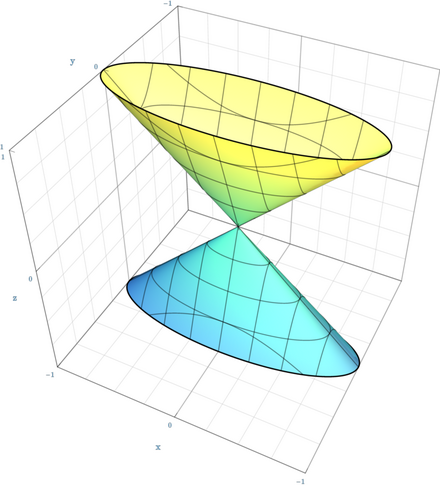
\includegraphics[width=0.7\linewidth]{divisor}
			\caption{$xy=z^2$}
			\label{fig:divisor}
		\end{figure}
		
		\item $X$=$\frac{\Spec\C[x,y,z,w]}{(xy-zw)}$. So $D=L=\{x=z=0\}$.
	\end{itemize}
\end{example}
\begin{defn}
	$D$ is \textbf{\textit{Q-Cartier}} if there exists $N$ such that $ND$ is Cartier.
\end{defn}
\begin{prop}[Regarding the last example]
	No multiple of $D_1$ is Cartier.
\end{prop}
\addcontentsline{toc}{section}{References}
\printbibliography
\end{document}